\clearpage
\section{Von Neumann Probability}

\label{sec:von_neumann_probability}

%In the introdutory section regarding Quantum Computation we could note that probabilities are an intrinsic part of quantum theory.

 
In the beginning on the $20^{th}$ century the nature of light was once again in the spotlight. The question whether light would be a particle (corpuscular theory), or a wave (undulatory theory), was posed throughout History. Newton, notoriously, considered light to be a particle and presented arguments such as the fact that light travels in a straight like, not bending when presented with obstacles, unlike waves, and gave an interpretation of the diffraction mechanism by resorting to a special medium (aether), where the light corpuscles could create a localized wave\cite{DiasdeDeus:1387968}. 

%figura difracção

The idea of light as a particle stood up until the $18^{th}$century as many scientists (Robert Hooke, Christian Huygens and Leonhard Euler to name a few) tried to explain contradictions found in corpuscular theory. This brought back the idea that light behaves like a wave. 

One of the most famous experiments that corroborates the undulatory theory is the Young's experiments ($19^{th}$ century), or the double-slit interferometer.

%figura double-slit
\begin{figure}[h]
\centering 

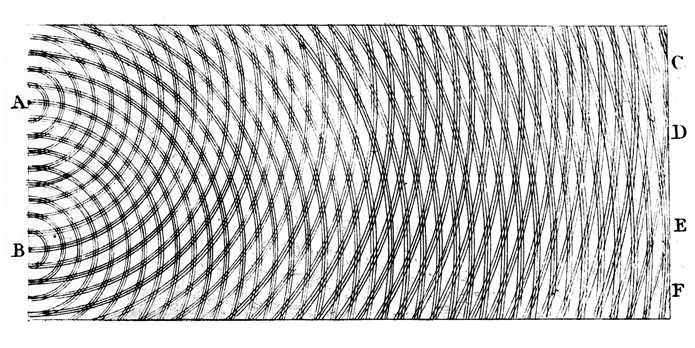
\includegraphics[scale=0.25]{Figures/Young_Diffraction.png}

\caption[Caption for LOF]
{Thomas Young's sketch of two-slit diffraction of light.} %\footnote}

\label{fig:double_slit}
\end{figure}
\footnotetext{Source: Young, Thomas: Probability. \url{http://en.wikipedia.org/wiki/File:Young_Diffraction.png (1803)}}

The apparatus for the double-slit experiment can be seen in Figure \ref{fig:double_slit}. A light source is placed in such a way that ``two portions" of light arrive at same time at the slits. Behind the barrier is a ``wall" placed to intercept the light. 
The light captured at a wall will sport an interference pattern similar to the pattern when two  waves interfere.
The double-slit experiment was considered for a while the full stop on the discussion on the nature of light.
However with experiments on the spectres of the light emitted by diverse substances and its relation with temperature, a new problem was posed. 

%figura black-body

The black body radiation problem was the theoretical problem where a body that absorbs light in all the electromagnetic spectrum, this makes the body acting as an natural vibrator, where each mode would have the same energy, according to the classic theory. 

When a black body is at a determined temperature the frequency of the radiation it emits depends on the temperature. The classic theory predicted that most of the energy of the body would be in the high frequency part of the spectrum (violet part) where most modes would be found, this led to a prediction called the ultraviolet catastrophe. According to the classic theory the black body would emit radiation with an infinite power for temperatures above approximately 5000K. 
Max Plank(1901), provided an explanation where the light was exchanged in discrete amounts called quanta, so that each frequency would only have specific levels of energy. Plank also determined through experimentation the value of the energy of the quanta that became known as photons later, that value became the physical constant called Plank constant:

\begin{equation}
\label{eq:plankconstant}
h = 6.62606957(29) \times 10^{-34} J.s
\end{equation}

In 1905, Einstein used the concept of quanta (photons) to explain the photoelectric effect. 
De Broglie(1924), suggested that all the matter had a wave-particle duality. This prediction was confirmed by studying the interference patterns caused by electron diffraction.


\subsection{Mathematical Foundations of Quantum Probability} 
\label{subsec:mathematical_foundations}

As previously explained, Quantum Theory is a branch of physics that has evolved from the need to explain certain phenomena that could not be explained with the current classical theory.
In the beginning of the 20\textsuperscript{th} century Dirac and von Neumann  helped to create the mathematical formalisms for this theory \cite{sep-qt-nvd}\cite{Summers2006}. 

Von Neumann's contributions were focused in the mathematical rigour, as is framework is strongly based in Hilbert's theory of operators. Dirac's concerns were more of a practical nature. Their combined contributions were invaluable to establish this area. 

From Dirac it is important to point the Dirac's notation (also known as Bra-ket notation or  $\langle Bra\vert c\vert ket\rangle$ ) (introduced in 1939 \cite{sep-qt-nvd}), that is widely used in literature based on quantum theory. This notation uses angle brackets and vertical bars to represent quantum states (or abstract vectors) as it can be seen in the formulas \eqref{rangle_dirac} and \eqref{langle_dirac}. 

\begin{equation}
\label{rangle_dirac}
\vert z\rangle = \left[\begin{array}{c}
z_{1}\\
z_{2}\\
...\\
z_{n}
\end{array}\right]
\end{equation}

\begin{equation}
\label{langle_dirac}
\langle z\vert= ( \vert z\rangle )^*  =\left[\begin{array}{cccc}
z_{1}^{*} & z_{2}^{*} & ... & z_{n}^{*}\end{array}\right]
\end{equation}




%of two quantum states ($\langle \phi \vert \psi \rangle$)
This notation provides for an elegant representation of the inner product \eqref{eq_inner} and verifies the has linearity as it follows in equation \eqref{eq_linearity}. While the Bra-ket notation can be useful in terms of condensing information, using vectors and matrices to represent the states turns out to be a more approachable way to understand and manipulate data.
 

\begin{equation}
\label{eq_inner}
\langle z\vert z\rangle={\displaystyle \sum_{i=1}^{n}\bar{z_{i}}z_{i}}
\end{equation}
where $\bar{z_{i}}$ is the complex conjugate of $z_{i}$.

 

\begin{equation}
\label{eq_linearity}
\langle z\vert(\alpha\vert x\rangle+\beta\vert y\rangle)=\alpha\langle z\vert x\rangle+\beta\langle z\vert y\rangle
\end{equation}


\subsection{Born rule}
\label{subsubsec:bornrule}

The Born rule was formulated by Born in 1926. This law allows to predict the probability that a measurement on a quantum system will yield a certain result. This law provides a link between the mathematical foundation of Quantum Mechanics and the experimental evidence\cite{VanRijsbergen2004}\cite{Landsman2009}. 

A quantum system is represented by a $n$-dimensional Hilbert Space, a complex vector space in which the inner product is defined. 




\begin{figure}[h]
\centering 

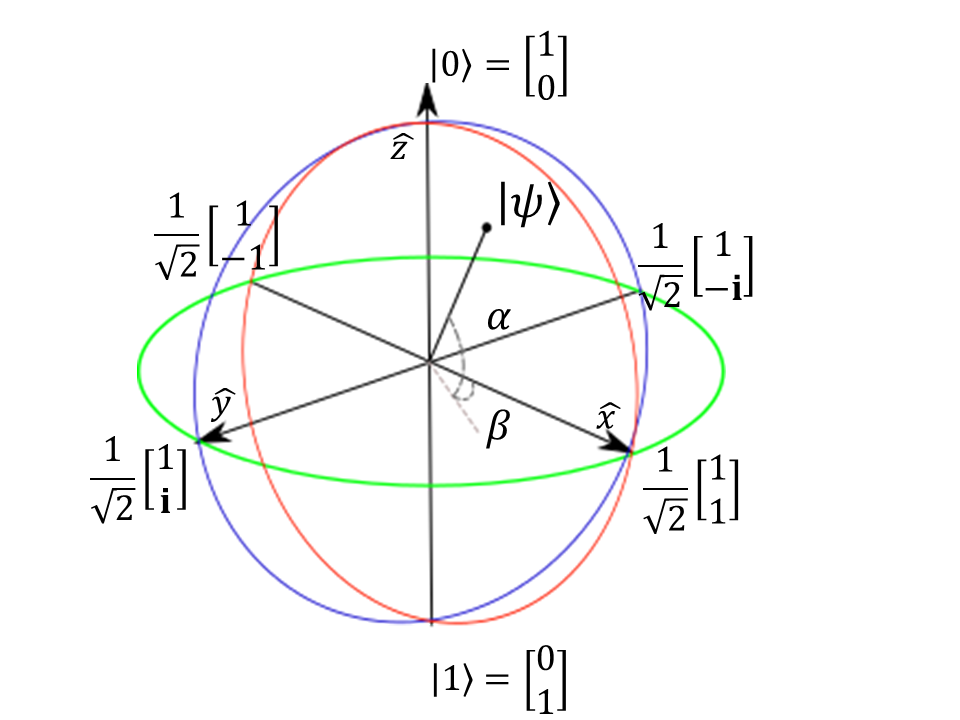
\includegraphics[scale=0.35]{Figures/bloch_sphere.png}
\caption{Representation of a two-dimensional Hilbert Space($\mathcal{H}^{2}$)}
\label{fig:circle}
\end{figure}


A $2$-dimensional Hilbert Space (corresponding to a qubit for example), can be represented by a Bloch Sphere. In the Figure \ref{fig:circle} we have a representation of quantum state $\vert v \rangle$ in a two-dimensional Hilbert Space. 



The Born rule states that if there is a system is in a state $\vert v \rangle$  (in a given $n$-dimensional Hilbert Space $\mathcal{H}$ ), and an Hermitian operator $A$ is applied then the probability of measuring a specific eigenvalue $\lambda_{i}$ associated with the $i$-th eigenvector of $A$ ($\psi_{i}$), will be given by\cite{VanRijsbergen2004}: 


\begin{equation}
\label{eq_born_rule}
P_{v}(\lambda_{i}) = \langle v\vert Proj_{i}\vert v\rangle
\end{equation}

where $Proj_{i}$ is a projection matrix corresponding to $\psi_{i}$ :

 \begin{equation}
\label{eq_born_rule_1}
Proj_{i} = \vert\psi_{i}\rangle \langle \psi_{i}\vert
\end{equation}

Given the properties of A, the set of eigenvectors $\{ \psi_{1}, \psi_{2}, ..., \psi_{i},..., \psi_{n}\}$ forms a orthogonal basis of the $n$-dimensional Hilbert Space considered. Thus the state $\vert v \rangle$
can be written as a linear combination of the eigenvectors of A:

 \begin{equation}
\label{eq_born_rule_lala}
\vert v \rangle = \alpha_{1}\psi_{1}+ \alpha_{2}\psi_{2}+ ...+\alpha_{i}\psi_{i}+...+\alpha_{n}\psi_{n}
\end{equation}

The coefficients $\alpha_{i}$ are complex numbers called probability amplitudes, and their squared sum is equal to 1: 
\begin{equation}
\sum_{i=0}^{n} \vert \alpha_{i}\vert^{2} = 1
\end{equation}

this brings us to: 

\begin{equation}
\label{eq_born_rule_2}
P_{v}(\lambda_{i}) =\langle v\vert\psi_{i}\rangle\langle\psi_{i}\vert v\rangle=\vert\langle v\vert\psi_{i}\rangle \vert^{2} = \vert \alpha_{i}^{*}\alpha_{i}\vert^{2}
\end{equation}

So the determination of the probability of an event ($P(A)$ ),
is made by projecting the quantum state on the eigenvectors corresponding to the operator $A$ of the
Hilbert Space and measuring the squared length of the projection.\cite{Trueblood}
\begin{equation}
P(A)=\left(Proj_{A}\vert z\rangle\right)^{2}
\end{equation}
Applying an operator can be seen as applying a rotation matrix on the system ($\vert v \rangle$) and measuring the projection of $\vert v \rangle$ onto the imaginary axis and the real axis (Figure \ref{fig:circle}), or considering that we have a determined state vector and rotating the orthogonal basis of the Hilbert Space according to an operator and then to do a projection on the new chosen orthogonal basis.

According to Leiffer\cite{Leifer2008} ``quantum theory can be thought of as a non-commutative, operator-valued, generalization of classical probability theory". 

%traces and density operators

As in the classical probability theory where from a random variable it is possible to establish a probability distribution, also known as density function, in the Hilbert space there is a equivalent density operator.
The density operator ($\rho$) is a Hermitian operator that has the particularity of having its trace equal to 1\cite{VanRijsbergen2004}.

\begin{equation}
\label{eq_trace1}
\rho = \sum_{i=0}^{n} \alpha_{i} \vert\psi_{i}\rangle\langle\psi_{i}\vert
\end{equation} 

\begin{equation}
\label{eq_trace1}
tr( \rho ) = 1
\end{equation}

%proofed

\subsubsection{L\"{u}ders Rule}
\label{subsubsec:ludersrule}
L\"{u}ders Rule defines the state of a quantum system after a partial measurement. We can establish a parallel between this selective measurement and conditional probability\ref{subsubsec:conditionalprobability}\cite{Busch2009}.

To measure the state of a system we first use a projection operator on the quantum state. This is also the first stage of applying L\"{u}ders Rule\ref{eq:luders1}.

\begin{equation}
\label{eq:luders1}
A=Proj_{A}\vert s\rangle
\end{equation}

After the measurement the resulting state is normalized\ref{eq:luders2}.

\begin{equation}
\label{eq:luders2}
\vert s_{A}\rangle=\frac{A}{\vert A\vert}
\end{equation}

%proofed
\subsection{Example of the double-slit experiment with electrons}
\label{subsubsec:double_slit}
 Like the Young's Experiment with light created an interference pattern similar to a wave, firing electrons one at the time produces a similar pattern. The unobserved fired electron behaved like a wave and after passing the slits the wavelets interfered with one another to create a interference pattern. However if a measuring device was active while the electron was fired the interference pattern wasn't registered. 

\begin{figure}[h]
\centering 
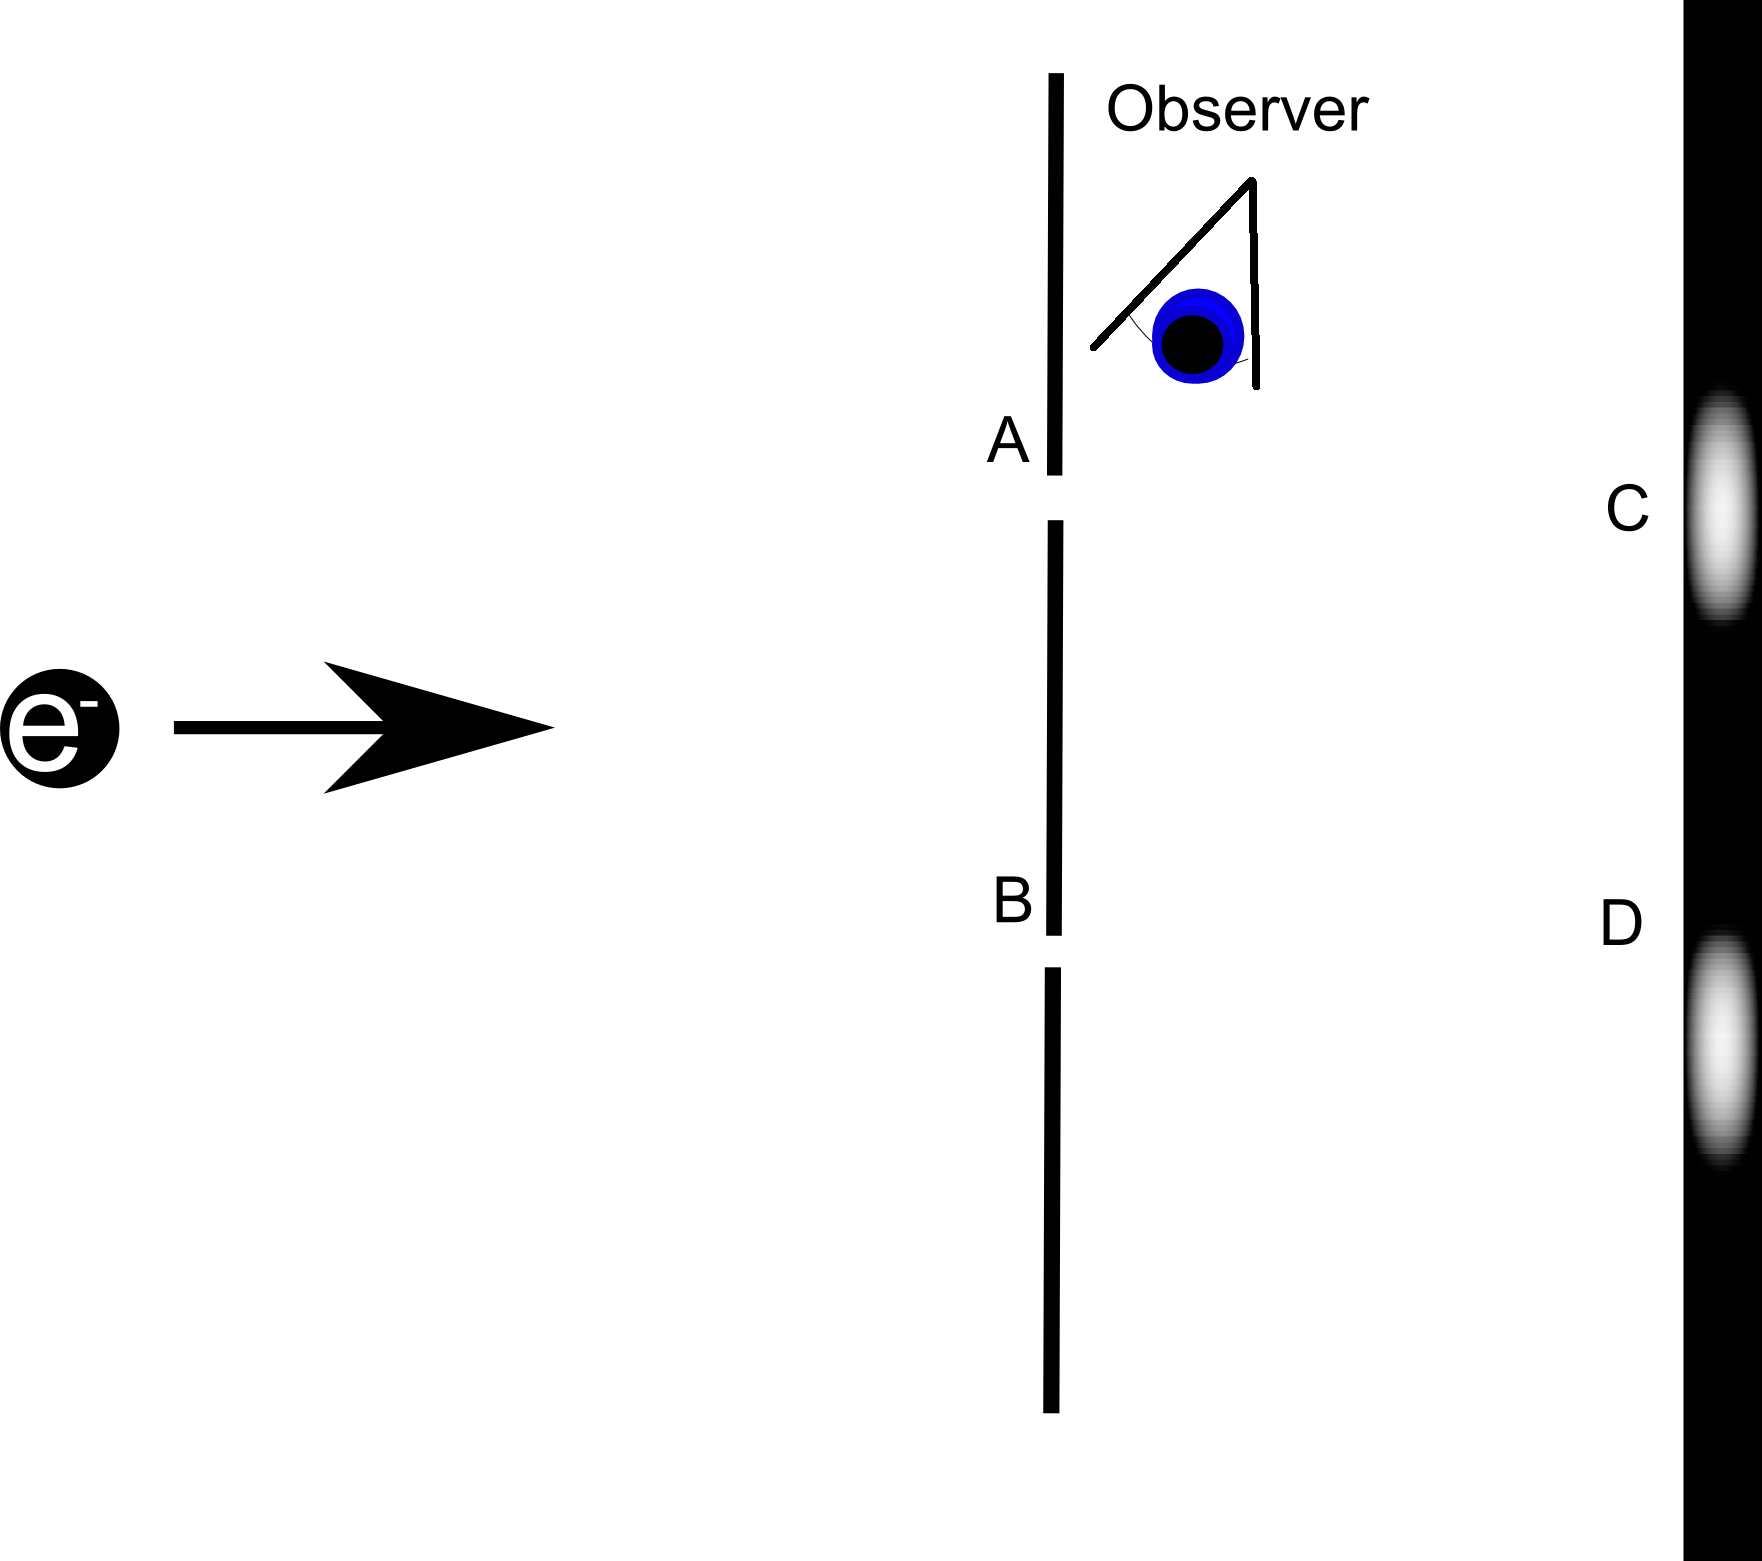
\includegraphics[scale=0.15]{Figures/ds_ob.png}
\caption{Double-slit experiment where there is a measuring device that allows to know through which slit the electron passed.}
\label{fig:double_slit_ob}

\end{figure}
\begin{figure}[h]
\centering 

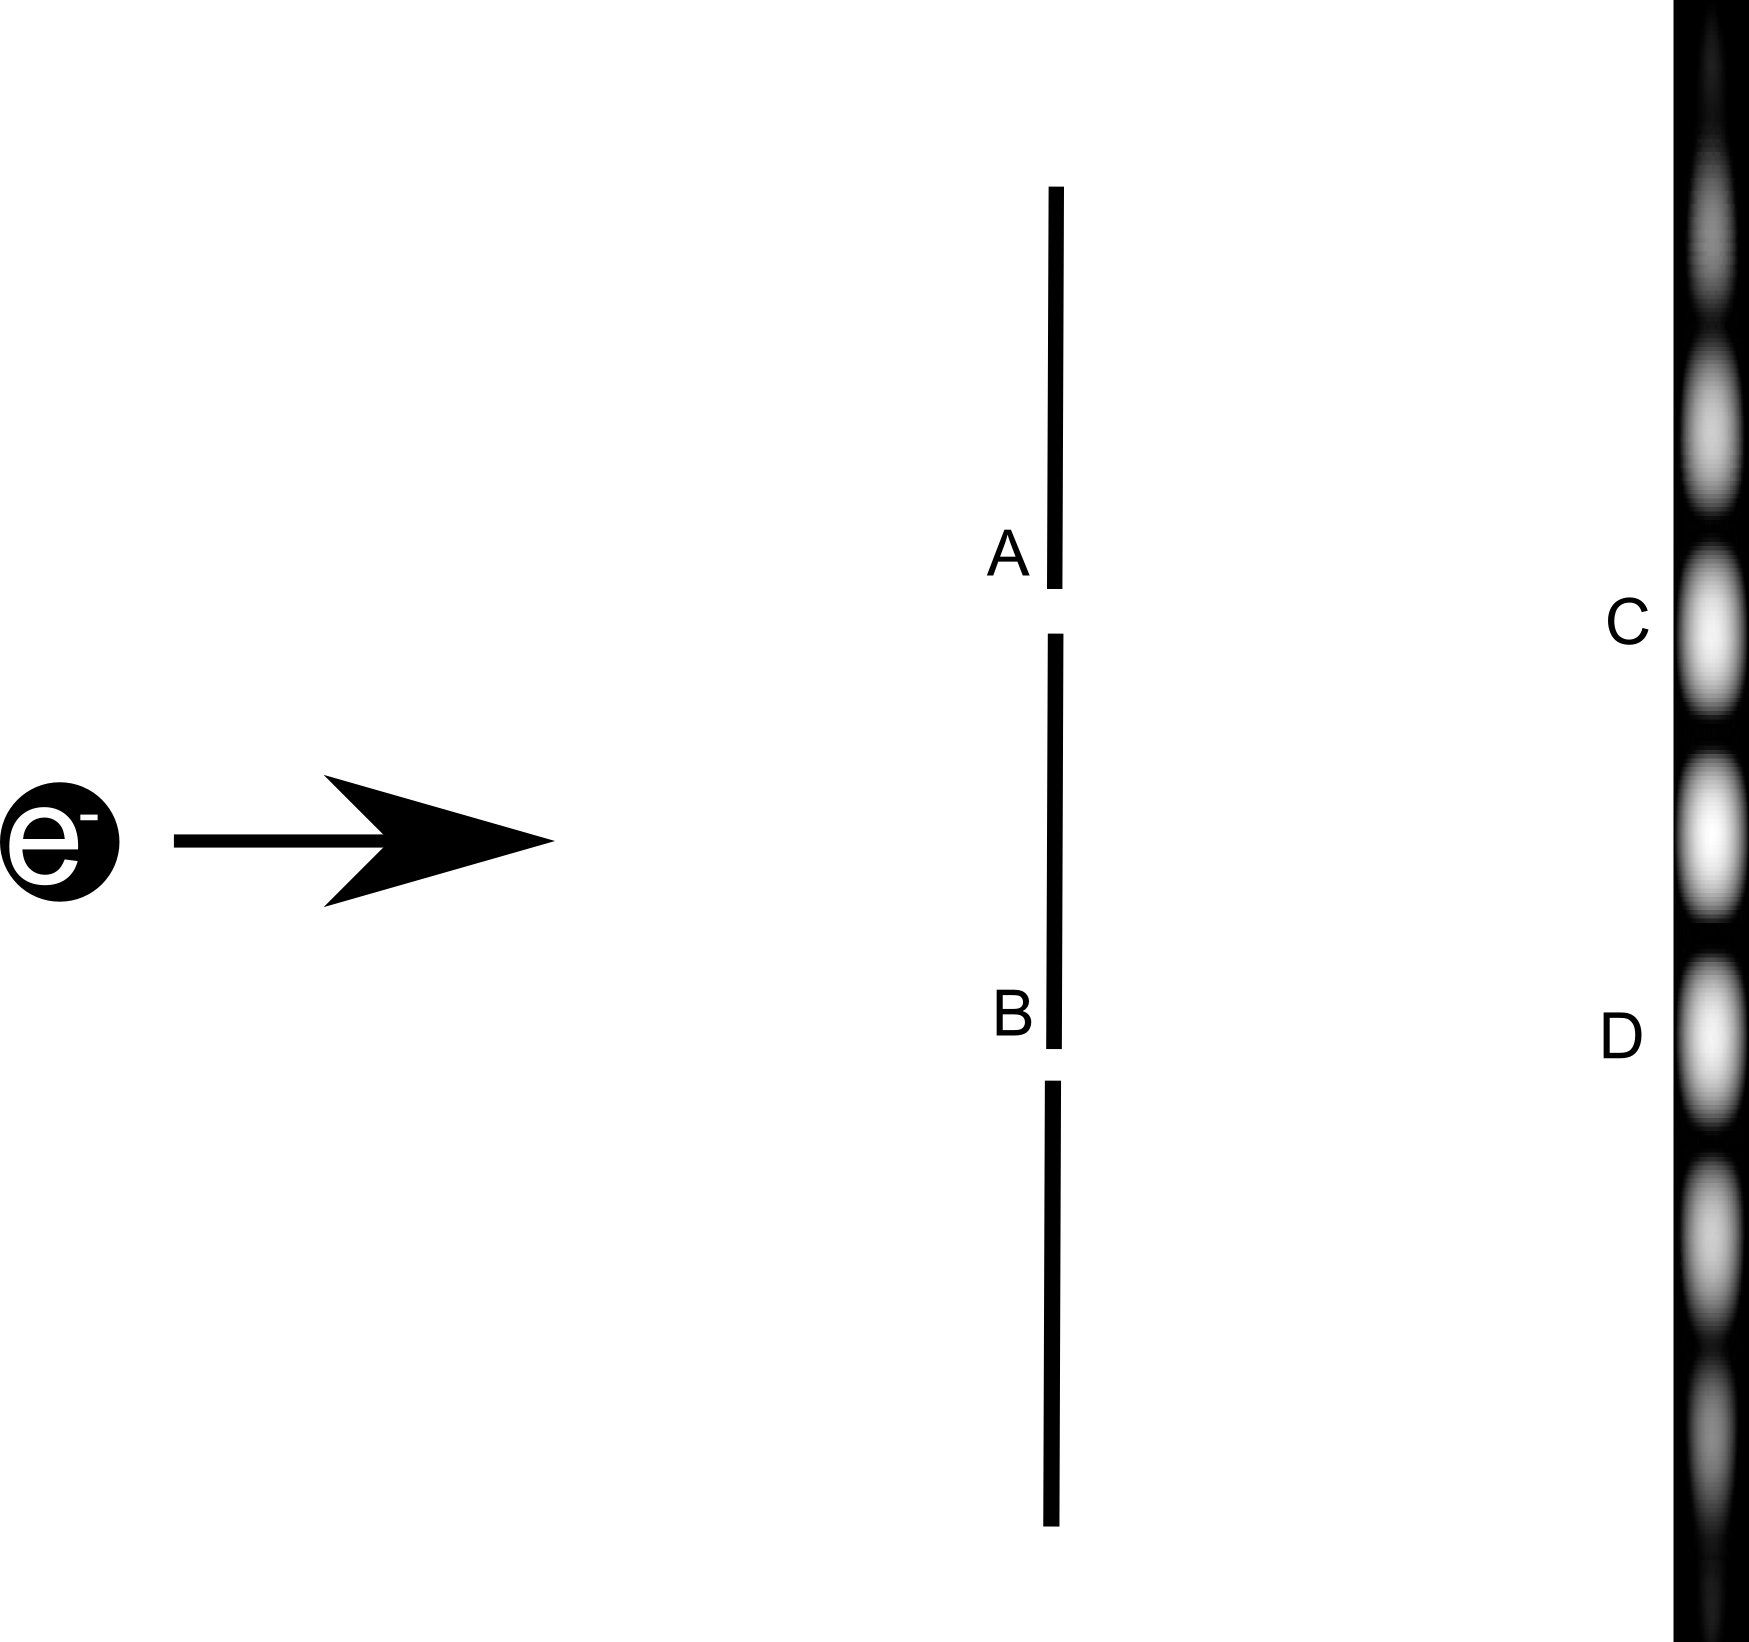
\includegraphics[scale=0.15]{Figures/ds_unob.png}
\caption{Double-slit experiment, where electrons exhibit the interference pattern characteristic in waves}
\label{fig:double_slit_unob}
\end{figure}

The fact that the electron was measured while passing through a slit produced a particle behaviour, explained by the classical theory (Figure \ref{fig:double_slit_ob}). 


In this experiment a single electron is shoot at a time. So in the start of the experiment (S), we know the initial position of the electron.

A final measurement (F) is made when the electron hits the wall behind the slits, where we know the final position of the electron.
\footnote{Mohrhoff, U.: Two Slits. \url{http://thisquantumworld.com/wp/the-mystique-of-quantum-mechanics/two-slit-experiment/##fn1back}}

If this experiment is observed, there is an intermediate measure that tells us whether the electron went through the slit A or B. The corresponding probability amplitudes related to this measurement are $\omega_{A}$ and $\omega_{B}$, and:
\begin{equation}
\omega_{A} = \langle F \vert A\rangle \langle A \vert S\rangle
\end{equation}
\begin{equation}
\omega_{B} = \langle F \vert B\rangle \langle B \vert S\rangle
\end{equation}

If we consider the intermediate measurement the probability $P(F\vert S)$ will be:
\begin{equation}
P(F\vert S) = 
\vert \langle F \vert A\rangle \langle A \vert S\rangle \vert^{2}
+
\vert \langle F \vert B\rangle \langle B \vert S\rangle \vert^{2}
\end{equation}

But if we only measure the position of the electron at the end of the experiment that probability will be:
\begin{equation}
P(F\vert S) = 
\vert \langle F \vert A\rangle \langle A \vert S\rangle 
+
 \langle F \vert B\rangle \langle B \vert S\rangle \vert^{2}
\end{equation}
The latter equation will be dependent on a interference coefficient that will be responsible the interference pattern observed in the unobserved experiment.



\subsection{Example of the Polarization of Light}
The photons in a beam of light don't vibrate all the same direction in most of the natural sources of light. To filter the light polaroids are used. A polaroid only allows the passage of light in a well-defined direction and thus reducing the intensity of the light. In the Figure \ref{fig:polaroids} we can observe that the introduction of the oblique polaroid in the third situation led to a passage of light. Although there is a classical explanation to this phenomenon if we consider waves when we are considering a beam of light, if our light source emits one photon at the time a quantum mechanical explanation is needed\cite{Rieffel2011}.

\begin{figure}[h]
\centering 

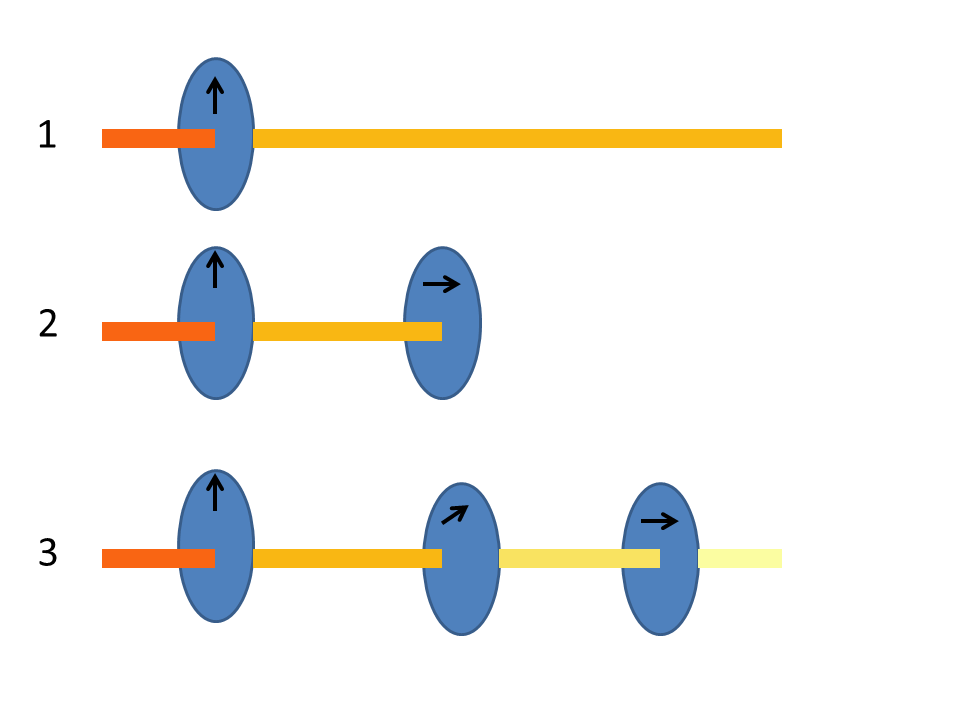
\includegraphics[scale=0.25]{Figures/Polaroids.png}
\caption{1. With one vertical polaroid the unpolarized light is attenuated by a half. 2. Vertical polarization followed by a horizontal polarization will block all the passing light. 3. Inserting a oblique polaroid between the vertical and horizontal polaroids will allow light to pass.}
\label{fig:polaroids}
\end{figure}

To model the polarization of the photon in a quantum setting, we will use a vector $\vert v \rangle $ in a two-dimensional Hilbert Space: 
\begin{equation}
\vert v \rangle = a\left[\begin{array}{c}
1\\
0
\end{array}\right]+ b\left[\begin{array}{c}
0\\
1
\end{array}\right]
\end{equation}

where $\left[\begin{array}{c}
1\\
0
\end{array}\right]$ would represent the vertical direction (could also be represented by the state vector $\vert\uparrow\rangle$), and $\left[\begin{array}{c}
0\\
1
\end{array}\right] $ the horizontal one (another possible representation to this basis could be $\vert\rightarrow\rangle$). We can consider the Figure \ref{fig:circle} as a graphical representation for this system.

In the first situation if $a = \frac{1}{\sqrt{2}}$, that would mean that the probability of passing the vertical polaroid would be $a = (\frac{1}{\sqrt{2}})^{2} = 0.5$, that would light to the expected reduction of a half of the intensity of light. After passing through the vertical polaroid the photon will have a polarization of $\vert v \rangle = a\left[\begin{array}{c}
1\\
0
\end{array}\right]$. Considering now the second situation after we have our photon polarized vertically (like in the end on the first situation), the probability of being vertically polarized is 1, thus making the probability of passing through the horizontal polaroid 0.
In the third situation, after being vertically polarized the photon will pass through an oblique polaroid that makes its direction

\begin{equation}
\vert v \rangle =  cos(\theta)\left[\begin{array}{c}
1\\
0
\end{array}\right]+ i.sen(\theta)\left[\begin{array}{c}
0\\
1
\end{array}\right]
\end{equation}



$\theta$ being the angle of the polaroid. The photon filtered by the vertical polaroid will pass this second polaroid with a probability of $(cos(\theta))^{2}$, becoming polarized according to the filter, as we can observe depending on the value of $\theta$ we will now have a horizontal component in the vector that describes the state of the photon. This will make the photon pass the horizontal polaroid  with a probability of $i.sen(\theta)^{2}$. 
%\nearrow




















